
\subsection{Дубликаты}

% Понятие «нечеткий дубликат» означает неполное или частичное
% совпадение текущего документа (изображения) с другим документом
% подобного класса.

% Дубликаты бывают естественные и искусственные.
% Естественные дубликаты --- схожие объекты, при схожих условиях.
% Искусственные нечеткие дубликаты --- полученные
% на основе одного и того же оригинала.
%
% Поиск нечетких дубликатов может быть полезен
% для оптической навигации беспилотных аппаратов,
% для определения характера ландшфта местности,
% составления каталогов видео,
% группировки сниппетов поисковых систем,
% фильтрация видео рекламы,
% и поиска пиратского видео.

\begin{frame}{Что такое <<нечеткие дубликаты>>}
    \begin{tabular}{ccccc}
        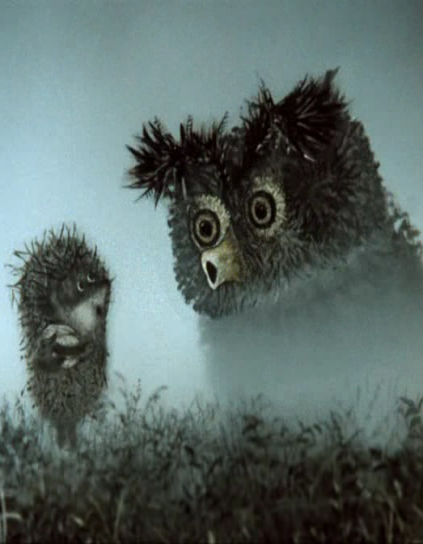
\includegraphics[height=4cm]{img/video/near-dublicate-1-1.png}
        &
        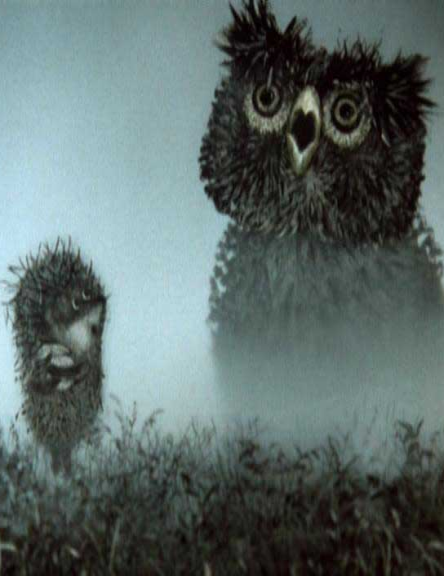
\includegraphics[height=4cm]{img/video/near-dublicate-1-2.png}
        &
        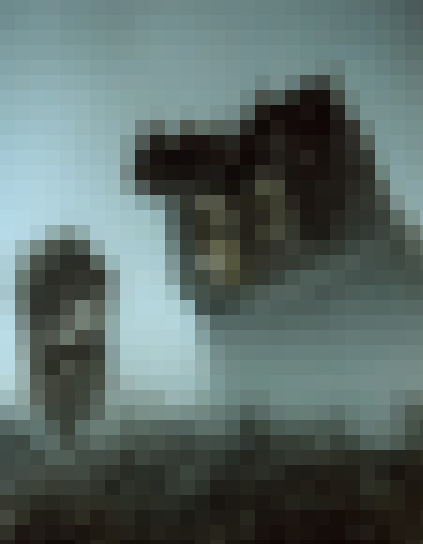
\includegraphics[height=4cm]{img/video/near-dublicate-1-3.png}
        \\
        {\small оригинал}
        &
        {\footnotesize естественный дубликат}
        &
        {\footnotesize искусственный дубликат}
        \\
    \end{tabular}
\end{frame}
